\section{Appendix}
\subsection{Requirements}
\textbf{Server}
\begin{itemize}
\item Must support one or more WCF services, written in C\#
\item Must be deployed on a IIS 7 Server
\item Must use a Microsoft SQL database
\item Must support multiple users using the same media file concurrently
\item Must support both admin and normal user login(by either facebook or
google), which gives different privileges
\item Must support handling of both upload, rent, and download of files
\item Must support search for media files in the database, based on arguments provided by the client
\item Must be able to process and distribute payments between users and \item authors. 
\item Must hold meta information about each media files, which is displayed at the client application (more analytic information)
\item Based on a user’s previous rented or downloaded files, the server must be able to show recommendations
\item Must give users the option to rate a tutorial
\item The server will provide the user the option to choose what kind of knowledge he or she have. 
\end{itemize}
\vspace{10pt}

\textbf{Client}\\
\textbf{Use-cases}\\
\textbf{1\#}\\
User A wants to login to use the RentItClient and must provide his credentials.
Precondition: Has a running computer and a working internet connection
Postcondition: Is logged in to the site
\begin{enumerate}
\item Opens the Chrome browser
\item Enters the URL to the website
\item Is presented with the homepage and navigates to the login form
\item Enters his credentials
\end{enumerate}

\vspace{10pt}
\textbf{2\#}\\
User A has made a video tutorial and wants to upload this to the server
Precondition: Is logged into the site
Postcondition: Has uploaded a video
\begin{enumerate}
\item Navigates to the upload button and presses this
\item Is presented with a form, where its possible to browse through files
\item Finds and selects the video
\item User A fills out forms about description, tagging and categorizing.
\item Uploads the video by pressing the ‘OK’ button. 
\end{enumerate}

\vspace{10pt}
\textbf{3\# }\\
User B wants to learn something about a special topic and searches for this using the RentItClient. 
Precondition: Is logged into the site.
Postcondition: Is able to view the video
\begin{enumerate}
\item Navigates to the ‘category’ section and is presented with a list of categories. 
\item Finds the category he likes and selects that.
\item Scrolls in a list of videos and selects the one he finds interesting. 
\item Can either choose to rent or buy the video.
\item Get an URL address and gets the video
\end{enumerate}

\vspace{10pt}
\textbf{4\# }\\
User B wants to see a video and downloads this to his computer
Precondition: Is logged in and authenticated by the server 
Postcondition: The video is downloaded to the computer
\begin{enumerate}
\item Navigates to the search form and types in a search string
\item Is presented with the results
\item Can select between the results and selects the one he wants
\item Can either choose to rent or buy the video and chooses to buy
\item Chooses where the file should be saved
\item Pays for the video and is given a download link
\item The download starts
\end{enumerate}

	
\vspace{10pt}
\textbf{5\# }\\
User A wants to see a tutorial, but does not want to keep this on his computer, so he only rents the video
Precondition: Is logged in and authenticated by the server
Postcondition: Has received a link to the video
\begin{enumerate}
\item Navigates to the search form and types in a searchstring
\item Is presented with the results
\item Can select between the results and selects the one he wants
\item Can either choose to rent or buy the video and chooses to rent
\item Pays for the video and is given a download link
\item The video is displayed.
\end{enumerate}
	
\vspace{10pt}
\textbf{6\#}\\
John Doe has heard about the RentItClient and wants to learn cool stuff
Precondition: Has a working internet connection
Postcondition: Is created as a user in the site.
\begin{enumerate}
\item Enters the URL to the site
\item Navigates to the ‘Create User’ form
\item Can either choose to create a user only used at this site or login using Facebook credentials
\item Types in a username and password and presses a ok button. 
\end{enumerate}

\vspace{10pt}
\textbf{7\#}\\
User A liked a video tutorial and would like to rate it
Precondition: Has seen a video tutorial
Postcondition: Has rated the video tutorial
\begin{enumerate}
\item User has an active account
\item Sees video tutorial
\item Wants to give the tutorial 7 in rating
\item Types in 7 in a rating field and presses the rate button
\end{enumerate}


\vspace{10pt}
\textbf{8\#}\\
User C has found some incorrect information and needs to correct this
Precondition: Has uploaded a video that allegedly contains an error
Postcondition: Has corrected the error
\begin{enumerate}
\item User has an active account
\item User has uploaded a video
\item User wishes to change the content
\item User changes the content and saves the changes
\end{enumerate}
	

\vspace{10pt}
\textbf{9\#}\\
A user wishes to deposit money to his account
Precondition: The user has an active account
Postcondition: The user has deposited money to his account
\begin{enumerate}
\item The user goes to the account site
\item The user inserts account/card information and amount to insert
\item The chosen amount is inserted into the users account
\end{enumerate}
	


\vspace{10pt}
\textbf{10\#}\\
A user wishes to withdraw money from his account
Precondition: The user has an active account with money inserted into it
Postcondition: The user has withdrawn the chosen amount from his account
\begin{enumerate}
\item The user goes to the account site
\item The user inserts the amount to withdraw
\item The chosen amount is withdrawn from the users account
\end{enumerate}
	
\vspace{10pt}
\textbf{11\#}\\
A user wishes to pay for a video
Precondition: The user has an active account with money deposited
Postcondition: The chosen video is available to the user
\begin{enumerate}
\item The user find the video he wishes to buy
\item The user press the buy button and pays for the video
\item The user is granted access to the video
\end{enumerate}
\newpage

\textbf{Factor Table}\\
\begin{center}
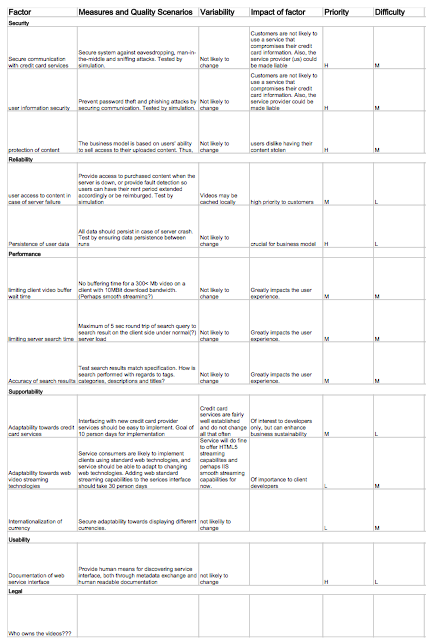
\includegraphics[scale=1.7]{FactorTable.png}
\end{center}
